У даному розділі наведено теоретичні засади підходу, який використовується для розв'язання мішаних задач теорії пружності для прямокутної області.
Він базується на зведенні вихідної задачі, шляхом застосування методу інтегральних перетворень, до одновимірної задачі у просторі трансформант.
Побудова матричної функції Гріна та розв'язання відповідних крайових задач надає можливість отримати аналітичний розв'язок поставленої задачі.
Матеріал цього розділу викладено у працях
\cite{pozhylenkov_1}, \cite{pozhylenkov_2}, \cite{pozhylenkov_3}, \cite{pozhylenkov_4}, \cite{pozhylenkov_5}, \cite{pozhylenkov_6}.

\subsection{Загальна постанова задачі}
\begin{figure}[h]
    \begin{center}
        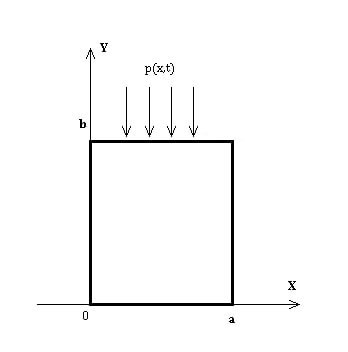
\includegraphics[scale=1]{images/geometry/image_4.jpg}
    \end{center}
    \caption{Геометрія задачі}\label{geom_gen}
\end{figure}
Розглядається пружний прямокутник (Рис: \ref{geom_gen}), який займає область, що у декартовій системі координат описується співвідношеннями $0 \le x \le a$, $0 \le y \le b$.

До прямокутної області по грані $y=b$ додане нормальне навантаження
\begin{equation}
    \sigma_y(x, y, t) |_{y=b} = -p(x, t), \quad  \tau_{xy}(x,y,t) |_{y=b} =0,
\end{equation}
де $p(x, t)$ відома функція, $t$ - час.
По нижній грані виконуються умови ідеального контакту
\begin{equation}
    v(x,y,t) |_{y=0}, \quad \tau_{xy}(x,y,t) |_{y=0} =0
\end{equation}
На бічних гранях $x=0$ та $x=a$ граничні умови подано у формі
\begin{equation}\label{gen_bound_gen}
    U_1[f(x,y,t)]=0, \quad U_2[f(x,y,t)]=0 ,
\end{equation}
де 
\begin{align*}
    &U_1[f(x,y,t)]=\left[\alpha_1f(x,y,t) + \beta_1 \frac{\partial f(x,y,t)}{\partial x} \right]|_{x=0}, \\
    &U_2[f(x,y,t)]=\left[\alpha_2f(x,y,t) + \beta_2 \frac{\partial f(x,y,t)}{\partial x} \right]|_{x=a}, \\
\end{align*}
- граничні функціонали у загальному зображенні (для кожної конкретної задачі вони будуть деталізовані), $f(x,y,t)=(u(x,y,t), v(x,y,t))^T$ - вектор переміщеннь.

Переміщення усередині прямокутника мають задовільняти рівняння Ламе:
\begin{equation}
    \begin{cases}
        \frac{\partial^2 u(x,y,t)}{\partial x^2} + \frac{\partial^2 u(x,y,t)}{\partial y^2} + \mu_0 (\frac{\partial^2 u(x,y,t)}{\partial x^2} + \frac{\partial^2 v(x,y,t)}{\partial x\partial y}) = \frac{1}{c_1^2} \frac{\partial^2 u(x,y,t)}{\partial t^2} \\
        \frac{\partial^2 v(x,y,t)}{\partial x^2} + \frac{\partial^2 v(x,y,t)}{\partial y^2} + \mu_0 (\frac{\partial^2 u(x,y,t)}{\partial x \partial y} + \frac{\partial^2 v(x,y,t)}{\partial y^2}) = \frac{1}{c_2^2} \frac{\partial^2 v(x,y,t)}{\partial t^2} \\
    \end{cases}
\end{equation}

Тут і далі розглянуто постановки задач у випадку гармонічних коливань
\begin{equation}\label{garm_gen}
    u(x,y,t) = u(x,y) e^{i \omega t}, \quad v(x,y,t) = v(x,y) e^{i \omega t}, \quad p(x, y, t) = p(x, y) e^{i \omega t}
\end{equation}
З урахуванням подання переміщеннь \eqref{garm_gen} рівняння рівноваги переформульовано:
\begin{equation}\label{lame_gen}
    \begin{cases}
        \frac{\partial^2 u(x,y)}{\partial x^2} + \frac{\partial^2 u(x,y)}{\partial y^2} + \mu_0 (\frac{\partial^2 u(x,y)}{\partial x^2} + \frac{\partial^2 v(x,y)}{\partial x\partial y}) = -\frac{\omega^2}{c_1^2}  u(x,y) \\
        \frac{\partial^2 v(x,y)}{\partial x^2} + \frac{\partial^2 v(x,y)}{\partial y^2} + \mu_0 (\frac{\partial^2 u(x,y)}{\partial x \partial y} + \frac{\partial^2 v(x,y)}{\partial y^2}) = -\frac{\omega^2}{c_2^2} v(x,y) \\
    \end{cases}
\end{equation}
Граничні умови набувають вигляду:
\begin{equation}\label{bound_gen}
    \begin{cases}
        \sigma_y(x, y) |_{y=b} = -p(x), \quad  \tau_{xy}(x,y) |_{y=b} =0 \\
        v(x,y) |_{y=0}, \quad \tau_{xy}(x,y) |_{y=0} =0 \\
        U_1[f(x,y)]=0, \quad U_2[f(x,y)]=0
    \end{cases}
\end{equation}

% Введемо нові невідомі функції $\chi_1(y) = u(0, y)$, $\chi_2(y) = v(0, y)$, $\chi_3(y) = u(a, y)$, $\chi_4(y) = v(a, y)$.
% Враховучи умову \eqref{gen_bound_gen}, отримаємо, що 
% $\frac{\partial u(0, y)}{\partial x}=-\frac{\alpha_1}{\beta_1} \chi_1(y)$,
% $\frac{\partial v(0, y)}{\partial x}=-\frac{\alpha_1}{\beta_1} \chi_2(y)$,
% $\frac{\partial u(a, y)}{\partial x}=-\frac{\alpha_2}{\beta_2} \chi_3(y)$,
% $\frac{\partial v(a, y)}{\partial x}=-\frac{\alpha_2}{\beta_2} \chi_4(y)$.

Потрібно відшукати хвильове поле пружного прямокутника,
що задовольняє крайову задачу \eqref{lame_gen}, \eqref{bound_gen}.

\subsection{Зведення вихідної задачі до задачі у просторі трансформант}
Для зведення вихідної задачі до одновимірної задачі до рівняннь \eqref{lame_gen} застосовано інтегральне перетворення Фур'є за змінною $x$:
\begin{equation}\label{int_trans_gen}
    \begin{pmatrix}
        u_n(y) \\
        v_n(y)
    \end{pmatrix} = \int_{0}^{a} 
    \begin{pmatrix}
        u(x,y) sin(\alpha_n x) \\
        v(x,y) cos(\alpha_n x)
    \end{pmatrix} dx, \quad \alpha_n = \frac{\pi n}{a}
\end{equation}

Для цього перше та друге рівняння \eqref{lame_gen} помножено відповідно на $sin(\alpha_n x)$ та $cos(\alpha_n x)$ та проінтегровано за змінною $x$ на інтервалі $0 \le x \le a$.

Тоді у просторі трансформант маємо:
\begin{equation}\label{transf_gen}
    \begin{cases}
        u_n^{''}(y) - \alpha_n \mu_0 v_n^{'}(y) - (\alpha_n^2 + \alpha_n^2 \mu_0 - \frac{\omega^2}{c_1^2}) u_n(y) = \\
        = \alpha_n(1 + \mu_0)(\chi_3(y) cos(\alpha_n a) - \chi_1(y)) \\
        \\
        (1 + \mu_0) v_n^{''}(y) + \alpha_n \mu_0 u_n^{'}(y) - (\alpha_n^2 - \frac{\omega^2}{c_2^2}) v_n(y) = \\
        = (\frac{\alpha_2}{\beta_2}\chi_4(y) cos(\alpha_n a) - \frac{\alpha_1}{\beta_1}\chi_2(y)) - \mu_0 (\chi_3^{'}(y) cos(\alpha_n a) -\chi_1^{'}(y))
    \end{cases}
\end{equation}

Тут $\chi_1(y) = u(0, y)$, $\chi_2(y) = v(0, y)$, $\chi_3(y) = u(a, y)$, $\chi_4(y) = v(a, y)$.
Враховучи умову \eqref{gen_bound_gen}, отримаємо, що 
$\frac{\partial u(0, y)}{\partial x}=-\frac{\alpha_1}{\beta_1} \chi_1(y)$,
$\frac{\partial v(0, y)}{\partial x}=-\frac{\alpha_1}{\beta_1} \chi_2(y)$,
$\frac{\partial u(a, y)}{\partial x}=-\frac{\alpha_2}{\beta_2} \chi_3(y)$,
$\frac{\partial v(a, y)}{\partial x}=-\frac{\alpha_2}{\beta_2} \chi_4(y)$.

Після застосування інтегрального перетворення \eqref{int_trans_gen} до крайових умов \eqref{bound_gen}
отримано подання крайових умов у просторі трансформант:
\begin{equation}\label{transf_bound_gen}
    \begin{cases}
        \left( (2G + \lambda)v_n^{'}(y) + \alpha_n \lambda u_n(y) \right)|_{y=b} = -p_n, \\
        \left(u_n^{'}(y) - \alpha_n v_n(y)  \right)|_{y=b} = 0, \\
        v_n(y)|_{y=0} = 0, \\
        \left(u_n^{'}(y) - \alpha_n v_n(y)  \right)|_{y=0} = 0,
    \end{cases}
\end{equation}
де $p_n = \int_{0}^{a} p(x) cos(\alpha_n x) dx$.

Для того щоб розв'язати задачу у простосторі трансформант, її переписано у векторній формі.
\begin{align}\label{transf_mat_gen}
    &L_2\left[ Z_n(y) \right] = F_n(y),
\end{align}
де $L_2$ - диференціальний оператор другого порядку
\begin{align}
    &L_2\left[ Z_n(y) \right] = A * Z_n^{''}(y) + B * Z_n^{'}(y) + C * Z_n(y), 
\end{align}
\begin{equation*}
    A = \begin{pmatrix}
        1 & 0 \\
        0 & 1 + \mu_0
    \end{pmatrix}, \quad
    B = \begin{pmatrix}
        0 & -\alpha_n \mu_0 \\
        \alpha_n \mu_0 & 0
    \end{pmatrix}
\end{equation*}
\begin{equation*}
    C = \begin{pmatrix}
        -\alpha_n^2 -\alpha_n^2 \mu_0 + \frac{\omega^2}{c_1^2} & 0 \\
        0 & -\alpha_n^2 + \frac{\omega^2}{c_2^2}
    \end{pmatrix}, \quad
    Z_n(y) = \begin{pmatrix}
        u_n(y) \\
        v_n(y)
    \end{pmatrix},
\end{equation*}
\begin{equation*}
    F_n(y) = \begin{pmatrix}
        \alpha_n(1 + \mu_0)(\chi_3(y) cos(\alpha_n a) - \chi_1(y)) \\
        (\frac{\alpha_2}{\beta_2}\chi_4(y) cos(\alpha_n a) - \frac{\alpha_1}{\beta_1}\chi_2(y)) - \mu_0 (\chi_3^{'}(y) cos(\alpha_n a) -\chi_1^{'}(y))
    \end{pmatrix}
\end{equation*}
Граничні умови \eqref{transf_bound_gen} записано у зображенні:
\begin{align}\label{transf_bound_mat_gen}
    &U_i\left[ Z_n(y) \right] = D_i,
\end{align}
де $i = \overline{0, 1}$, $b_0 = b$, $b_1 = 0$
\begin{align}
    &U_i\left[ Z_n(y) \right] = E_i * Z_n^{'}(b_i) + F_i * Z_n(b_i),
\end{align}
\begin{equation*}
    E_0 = \begin{pmatrix}
        1 & 0 \\
        0 & 2G + \lambda
    \end{pmatrix}, \quad
    F_0 = \begin{pmatrix}
        0 & -\alpha_n \\
        \alpha_n \lambda & 0
    \end{pmatrix}, \quad
\end{equation*}
\begin{equation*}
    E_1 = \begin{pmatrix}
        1 & 0 \\
        0 & 0
    \end{pmatrix}, \quad
    F_1 = \begin{pmatrix}
        0 & -\alpha_n \\
        0 & 1
    \end{pmatrix}, \quad
\end{equation*}
\begin{equation*}
    D_0 = \begin{pmatrix}
        0 \\
        -p_n
    \end{pmatrix}, \quad
    D_1 = \begin{pmatrix}
        0 \\
        0
    \end{pmatrix} \quad
\end{equation*}

Розв'язок векторної одновимірної крайової задачі знайдено як суперпозиція загального розв'язку векторного однорідного рівняння $Z_n^0(y)$
та часткового розв'язку неоднорідного рівняння $Z_n^1(y)$.
\begin{equation}
    Z_n(y) = Z_n^0(y) + Z_n^1(y)
\end{equation}

Ці розв'язки знайдено за допомогою апарату матричного диференціального числення \cite{popov_4}, \cite{gantmaher},
для чого побудовано фундаментальну матричну систему розв'язків та фундаментальну базисну систему розв'язків відповідної матричної крайової задачі.

Як показано у \cite{popov_4} для знаходження розв'зку однорідного векторного рівняння \eqref{transf_mat_gen},
спочатку треба побудувати розв'язок матричного однорідного рівняння
\begin{equation}\label{hom_mat_trans_gen}
    L_2\left[ Y_n(y) \right] = 0
\end{equation}
де $Y_n(y)$ - матриця порядку $2\times2$.

Представимо матрицю $Y_n(y)$ у наступній формі $Y_n(y) = e^{sy}*I$, $I$ - одинична матриця, та підставимо до \eqref{hom_mat_trans_gen}.
В результаті отримаємо рівність $L_2\left[ e^{sy}*I \right] = e^{sy} * M(s)$, де матриця $M(s)$ має вигляд:
\begin{equation}
    M(s) = \begin{pmatrix}
        s^2 - \alpha_n^2 - \alpha_n^2\mu_0 + \frac{\omega^2}{c_1^2} & -\alpha_n \mu_0 s \\
        \alpha_n \mu_0 s & s^2 (1 + \mu_0) -\alpha_n^2 + \frac{\omega^2}{c_2^2}
     \end{pmatrix}
\end{equation}

Згідно до \cite{popov_5} розв'язок матричного однорідного рівняння побудовано у формі
\begin{equation}
    Y(y) = \frac{1}{2\pi i} \oint_C e^{sy} M^{-1}(s)ds
\end{equation}
де $M^{-1}(s)$ - матриця обернена до матриці $M(s)$, $C$ - замкнений контур який містить усі особливі точки матриці $M^{-1}(s)$.

Матрицю $M^{-1}(s)$ знайдено у наступному поданні $M^{-1}(s) = \frac{\widetilde{M(s)}}{det[M(s)]}$, де $\widetilde{M(s)}$ - транспонована матриця алгебричних доповнень,
$det[M(s)]$ - детермінант матриці, який знайдено як поліном четвертого ступеня
\begin{align}
    &det[M(s)] = \begin{vmatrix}
        s^2 - \alpha_n^2 - \alpha_n^2\mu_0 + \frac{\omega^2}{c_1^2} & -\alpha_n \mu_0 s \\
        \alpha_n \mu_0 s & s^2 (1 + \mu_0) -\alpha_n^2 + \frac{\omega^2}{c_2^2}
     \end{vmatrix} = \nonumber \\
    &=(s - s_1)(s + s_1)(s - s_2)(s + s_2)
\end{align}
де $s_1$, $s_2$, $-s_1$, $-s_2$ корені $det[M(s)]=0$, детальне знаходження яких наведено в Додатку В.

Обернена матриця має вигляд
\begin{align}
    &M^{-1}(s)= \frac{1}{(s - s_1)(s + s_1)(s - s_2)(s + s_2)} \nonumber \\
    &\begin{pmatrix}
        s^2 (1 + \mu_0) -\alpha_n^2 + \frac{\omega^2}{c_2^2} & \alpha_n \mu_0 s \\
        -\alpha_n \mu_0 s & s^2 - \alpha_n^2 - \alpha_n^2\mu_0 + \frac{\omega^2}{c_1^2}
    \end{pmatrix}
\end{align}
Враховучи це, знайдемо значення фундаментальної матриці за допомогою теореми про лишки:
\begin{align*}
    &\frac{1}{2\pi i} \oint_C e^{sy} M^{-1}(s)ds = \frac{2 \pi i}{2 \pi i (1 + \mu_0)} \sum_{i=1}^{4} Res\left[ e^{sy} \frac{\widetilde{M(s)}}{det[M(s)]} \right] = \\
    & = \left(Y_1(y) + Y_2(y) + Y_3(y) + Y_4(y) \right),
\end{align*}
де
\begin{align}\label{fund_mat_0_gen}
    &Y_0(y) =  \left( \frac{e^{sy}}{(s+s_1)(s - s_2)(s + s_2)} \widetilde{M(s)} \right) \Big|_{s=s_1} = \nonumber \\
    &=\frac{e^{s_1 y}}{2s_1 (s_1^2 - s_2^2)} \begin{pmatrix}
        s_1^2 (1 + \mu_0) -\alpha_n^2 + \frac{\omega^2}{c_2^2} & \alpha_n \mu_0 s_1 \\
        -\alpha_n \mu_0 s_1 & s_1^2 - \alpha_n^2 - \alpha_n^2\mu_0 + \frac{\omega^2}{c_1^2}
    \end{pmatrix}
\end{align}
\begin{align}\label{fund_mat_1_gen}
    &Y_1(y) =  \left( \frac{e^{sy}}{(s-s_1)(s - s_2)(s + s_2)} \widetilde{M(s)} \right) \Big|_{s=-s_1} = \nonumber \\
    &=-\frac{e^{-s_1 y}}{2s_1 (s_1^2 - s_2^2)} \begin{pmatrix}
        s_1^2 (1 + \mu_0) -\alpha_n^2 + \frac{\omega^2}{c_2^2} & -\alpha_n \mu_0 s_1 \\
        \alpha_n \mu_0 s_1 & s_1^2 - \alpha_n^2 - \alpha_n^2\mu_0 + \frac{\omega^2}{c_1^2}
    \end{pmatrix}
\end{align}
\begin{align}\label{fund_mat_2_gen}
    &Y_2(y) =  \left( \frac{e^{sy}}{(s+s_2)(s - s_1)(s + s_1)} \widetilde{M(s)} \right) \Big|_{s=s_2} = \nonumber \\
    &=\frac{e^{s_2 y}}{2s_2 (s_2^2 - s_1^2)} \begin{pmatrix}
        s_2^2 (1 + \mu_0) -\alpha_n^2 + \frac{\omega^2}{c_2^2} & \alpha_n \mu_0 s_2 \\
        -\alpha_n \mu_0 s_2 & s_2^2 - \alpha_n^2 - \alpha_n^2\mu_0 + \frac{\omega^2}{c_1^2}
    \end{pmatrix}
\end{align}
\begin{align}\label{fund_mat_3_gen}
    &Y_3(y) =  \left( \frac{e^{sy}}{(s-s_2)(s - s_1)(s + s_1)} \widetilde{M(s)} \right) \Big|_{s=-s_2} = \nonumber \\
    &=-\frac{e^{-s_2 y}}{2s_2 (s_2^2 - s_1^2)} \begin{pmatrix}
        s_2^2 (1 + \mu_0) -\alpha_n^2 + \frac{\omega^2}{c_2^2} & -\alpha_n \mu_0 s_2 \\
        \alpha_n \mu_0 s_2 & s_2^2 - \alpha_n^2 - \alpha_n^2\mu_0 + \frac{\omega^2}{c_1^2}
    \end{pmatrix}
\end{align}

\subsection{Побудова матричної функції Гріна}
Для побудови матриці-функції Гріна спочатку знайдено фундаментальні базисні матриці $\Psi_0(y)$, $\Psi_1(y)$, які мають задовільняти матричну крайову задачу \cite{popov_2}:
\begin{align}\label{psi_probl_gen}
    &L_2\left[ \Psi_i(y) \right] = 0, \nonumber \\
    &U_i\left[ \Psi_j(y) \right] = \delta_{j,i}, \quad j= \overline{0, 1}, i= \overline{0, 1}
\end{align}

Для цього їх вибрано у поданні:
\begin{equation}\label{psi_gen}
    \Psi_i(y) = \left( Y_0(y) + Y_1(y) \right) * C_1^i + \left( Y_2(y) + Y_3(y) \right) * C_2^i
\end{equation}
Тут матриці $Y_i(y)$, $i=\overline{0, 3}$ визначено формулами \eqref{fund_mat_0_gen}-\eqref{fund_mat_3_gen}, де $C_1^j$, $C_2^j$, $j=\overline{0, 1}$ невідомі матриці коєфіцієнтів, які знайдено з граничних умов \eqref{psi_probl_gen}
(покрокове знаходження наведено у Додатку С).

Для подальшого введемо наступні позначення для елементів матриць $\Psi_0(y)$, $\Psi_1(y)$:
\begin{equation*}
    \Psi_0(y) = \begin{pmatrix}
        \Psi_1^0(y) &  \Psi_2^0(y) \\
        \Psi_3^0(y) &  \Psi_4^0(y) 
    \end{pmatrix}, \quad 
    \Psi_1(y) = \begin{pmatrix}
        \Psi_1^1(y) &  \Psi_2^1(y) \\
        \Psi_3^1(y) &  \Psi_4^1(y) 
    \end{pmatrix}      
\end{equation*}

Таким чином матрицю Гріна можемо записати у вигляді:
\begin{equation}\label{grin_matrix_gen}
    G(y,\xi) = 
    \begin{cases}
        \Psi_0(y) * \Psi_1(\xi), \quad 0 \le y < \xi \\
        \Psi_1(y) * \Psi_0(\xi), \quad \xi < y \le b
    \end{cases}
\end{equation}

Для данної матриці Гріна виконано усі властивості, зокрема виконано однорідні граничні умови \eqref{transf_bound_mat_gen}
та задовільнено однорідне рівняння рівноваги у просторі трансформант \eqref{transf_mat_gen}:
\begin{equation*}
    L_2\left[  G(y, \xi) \right] = 0
\end{equation*}
\begin{equation*}
    U_0\left[ G(y, \xi) \right] = 0, \quad  U_1\left[ G(y, \xi) \right] = 0,
\end{equation*}

За допомогою функції Гріна \eqref{grin_matrix_gen} розв'язок неоднорідної векторної крайової задачі у просторі трансформант записано у поданні \cite{popov_2}
\begin{equation}
    Z_n(y) = \int_0^b G(y,\xi) F_n(\xi) d\xi + \Psi_0(y) * D_0 + \Psi_1(y) * D_1
\end{equation}

Введемо наступні позначення $G(y, \xi) = \begin{pmatrix}
    g_1(y,\xi) & g_2(y,\xi) \\
    g_3(y,\xi) & g_4(y,\xi)
\end{pmatrix}$, $F_n(y) = \begin{pmatrix}
    f_n^1(y) \\
    f_n^2(y)
\end{pmatrix}$. Враховуючи це, шукані функціі переміщень у просторі трансформант можна записати у формі
\begin{align}\label{transf_sol_u_gen}
    &u_n(y) = \int_0^b \left[g_1(y, \xi)f_n^1(\xi) + g_2(y, \xi)f_n^2(\xi) \right]d\xi - \psi_0^2(y) p_n
\end{align}
\begin{align}\label{transf_sol_v_gen}
    &v_n(y) = \int_0^b \left[g_3(y, \xi)f_n^1(\xi) + g_4(y, \xi)f_n^2(\xi) \right]d\xi - \psi_0^4(y) p_n
\end{align}

Фінальний розв'язок вихідної задачі отримано після застосування оберненного перетворення Фур'є до трансформант \eqref{transf_sol_u_gen}, \eqref{transf_sol_v_gen}
\begin{equation}\label{final_sol_u_gen}
    u(x,y) = \frac{2}{a} \sum_{n=1}^{\infty} u_n(y) sin(\alpha_n x), \quad \alpha_n = \frac{\pi n}{a}
\end{equation}
\begin{equation}
    v(x,y) = \frac{v_0(y)}{a} + \frac{2}{a} \sum_{n=1}^{\infty} v_n(y) cos(\alpha_n x), \quad \alpha_n = \frac{\pi n}{a}
\end{equation}

Знайдем тепер $v_0(y)$ розглянувши задачу у просторі трансформант \eqref{transf_gen}, \eqref{transf_bound_gen} при $n=0$, $\alpha_n = 0$
(детальний розв'язок наведено у Додатку D). Тоді остаточний розв'язок $v(x,y)$ набуває вигляду
\begin{align}\label{final_sol_v_gen}
    &v(x,y) = \frac{2}{a} \sum_{n=1}^{\infty} v_n(y) cos(\alpha_n x) - \psi_0(y) \frac{p_0}{a(2G + \lambda)} + \nonumber \\
    &+ \frac{1}{a(1+\mu_0)} \int_{0}^{b}g(y,\xi) [ (\frac{\alpha_2}{\beta_2}\chi_4(\xi) cos(\alpha_n a) - \frac{\alpha_1}{\beta_1}\chi_2(\xi)) - \nonumber \\
    & - \frac{\mu_0}{(1+\mu_0)} (\chi_3^{'}(\xi) cos(\alpha_n a) -\chi_1^{'}(\xi)) ] d\xi
\end{align}

Невідомі функції $\chi_i(y)$, $i=\overline{1, 4}$ що містяться у формулі розв'язку \eqref{final_sol_u_gen}, \eqref{final_sol_v_gen} знайдено для кожної конкретної постанови задачі окремо.

\subsection{Загальна схема розв'язку сінгулярного інтегрального рівняння}
Розглянемо випадок виконання граничних умов другої основної задачі теорії пружності на бічних гранях, в результаті кількість невідомих функцій скоротиться до однієї $f(y) = \frac{\partial v(x,y)}{\partial x}|_{x=a}$.
З цього отримаємо значення $f_n^1(\xi) = 0$, $f_n^2(\xi)= -cos(\alpha_n a) f(\xi)$.
Для знаходження невідомої функції $f(y)$ використано граничну умову $\sigma_y(x, y) |_{y=b} = -p(x)$ та побудовано сінгульрне інтегральне рівнняння:
\begin{equation}\label{int_eq_gen}
    \frac{1}{\pi} \int_{-1}^{1} \left( a_2(t) ln\left[ \frac{1}{\lvert x - t \rvert} \right] + a_3(t, x) \right) f(t) dt = a_1(x),
\end{equation}
де
% нужно поправить
\begin{align*}
    &a_1(x) = a p(x) - 2(2G + \lambda) \frac{\partial}{\partial y} \sum_{n=1}^{\infty} \psi_0^{4}(y) p_n cos(\alpha_n x)|_{y=b} - \nonumber \\
    &- 2\lambda \frac{\partial}{\partial x} \sum_{n=1}^{\infty}\psi_0^2(y) p_n sin(\alpha_n x)|_{y=b} - \psi_0^{'}(b) p_0
\end{align*}
\begin{equation*}
    a_2(t) = \frac{2}{\pi} \lim_{n \rightarrow \infty}\left[ \frac{\partial \widetilde{g_4(y, \xi)}}{\partial y} + \lambda \widetilde{g_2(y, \xi)} \right]|_{y=b}, 
\end{equation*}
\begin{align*}
    &a_3(t, x) = \sum_{n=1}^{N} cos(\alpha_n a) cos(\alpha_n x) \left[(2G + \lambda) \frac{\partial g_4(y, t)}{\partial y} + \alpha_n \lambda g_2(y, t) \right]|_{y=b} - \\
    & - a_2 \sum_{n=0}^{N} (-1)^n (2n + 1)^{-1} e^{-(2n + 1) \frac{\pi}{2a} (b - t)} cos((2n + 1) \frac{\pi}{2a} x)
\end{align*}

Інтегральне рівняння \eqref{int_eq_gen} розв'язується методом ортогональних поліномів \cite{popov_3}.
Згідно з методом невідому функцію $f(t)$ розвинуто у ряд за поліномами Чебишева першого роду
\begin{equation}\label{unk_fun_gen}
    f(t) = \frac{1}{a_2(t)} \frac{1}{\sqrt{1 - t^2}} \sum_{k=0}^{\infty} \varphi_k T_{k}(t),
\end{equation}
де $\varphi_k$ - невідомі коєфіцієнти, $T_{k}(t)$ - поліном Чебишева першого роду.

Представлення невідомої функції \eqref{unk_fun_gen} підставлено у сінгулярне інтегральне рівняння \eqref{int_eq_gen}
та враховуючи спектральне співвідношення B.1.9 \cite{ortogonal}
\begin{equation}
    \frac{1}{\pi} \int_{-1}^{1} ln\left[ \frac{1}{\lvert x - t \rvert} \right] \frac{T_k(t)}{\sqrt{1 - t^2}} dt = \upsilon_k T_k(x),
    \begin{cases}
        \upsilon_0 = ln 2, \\
        \upsilon_k = k^{-1}, k \ge 1
    \end{cases}
\end{equation} 
отримано
\begin{equation}\label{int_eq_2_gen}
    \sum_{k=0}^{\infty}  \varphi_k \upsilon_k T_{k}( x ) + \sum_{k=0}^{\infty} \varphi_k \frac{1}{\pi} \int_{0}^{1} \frac{a_3(t, x)}{a_2(t)} \frac{T_{k}(t)}{\sqrt{1 - t^2}} dt = a_1(x)
\end{equation}

Реалізація стандартної схеми методу ортогональних поліномів приводить до розв'язання нескінченої системи алгебричних рівнянь відносно невідномих коєфіцієнтів $\varphi_k$, $k=\overline{0, \infty}$,
яка в подальшому розв'язується методом редукції.

\begin{equation}\label{int_system_gen}
    \frac{\phi_m \pi}{2m} + \sum_{k=0}^{\infty} \phi_k g_{k, m} = f_m,
\end{equation}
де $g_{k, m} = \frac{1}{\pi} \int_{-1}^{1} \frac{T_{m}(x)}{\sqrt{1 - x^2}} \int_{0}^{1} \frac{a_3(t, x )}{a_2(t)} \frac{T_{k}(t)}{\sqrt{1 - t^2}} dt dx$,
$f_m = \int_{-1}^{1} \frac{T_{m}(x) a_1(x)}{\sqrt{1 - x^2}} dx$ інтеграли відомих функцій


% Запишемо тепер фінальний розв'язок для цього випадку:
% \begin{equation}
%     u(x,y) = -\frac{2}{a} \sum_{n=1}^{\infty} \left( \int_0^b \left[g_2(y, \xi)cos(\alpha_n a) f(\xi) \right]d\xi + \psi_0^2(y) p_n \right) sin(\alpha_n x)
% \end{equation}
% \begin{align}
%     &v(x,y) = -\frac{1}{a(1+\mu_0)} \int_{0}^{b}g(y,\xi) f(\xi) d\xi - \psi_0(y) \frac{p_0}{a(2G + \lambda)} \nonumber \\
%     &- \frac{2}{a} \sum_{n=1}^{\infty} \left( \int_0^b \left[g_4(y, \xi) cos(\alpha_n a) f(\xi) \right]d\xi + \psi_0^4(y) p_n  \right) cos(\alpha_n x)
% \end{align}

% Використиємо граничну умову $\sigma_y(x, y) |_{y=b} = -p(x)$ для того, щоб отримати інтегральне рівняння:
% \begin{equation*}
%     (2G + \lambda)\frac{\partial v(x,y)}{\partial y}|_{y=b} + \lambda\frac{\partial u(x,y)}{\partial x}|_{y=b} = -p(x) \Leftrightarrow
% \end{equation*}
% \begin{align*}
%     &-\frac{(2G + \lambda)}{a(1+\mu_0)} \int_{0}^{b}\frac{\partial g(y, \xi)}{\partial y}|_{y=b} f(\xi) d\xi - \psi_0^{'}(b) \frac{p_0}{a} - \\
%     &- \frac{2(2G + \lambda)}{a} \frac{\partial}{\partial y} \sum_{n=1}^{\infty} \left( \int_0^b \left[g_4(y, \xi) cos(\alpha_n a) f(\xi) \right]d\xi + \psi_0^{4}(y) p_n \right) \\ 
%     &cos(\alpha_n x)|_{y=b} - \frac{2\lambda}{a} \frac{\partial}{\partial x} \sum_{n=1}^{\infty} \left( \int_0^b \left[g_2(y, \xi)cos(\alpha_n a) f(\xi) \right]d\xi + \psi_0^2(y) p_n \right) \\ 
%     &sin(\alpha_n x)|_{y=b} = -p(x)
% \end{align*}
% Введемо позначення:
% \begin{align}
%     &a_1(x) = a p(x) - 2(2G + \lambda) \frac{\partial}{\partial y} \sum_{n=1}^{\infty} \psi_0^{4}(y) p_n cos(\alpha_n x)|_{y=b} - \nonumber \\
%     &- 2\lambda \frac{\partial}{\partial x} \sum_{n=1}^{\infty}\psi_0^2(y) p_n sin(\alpha_n x)|_{y=b} - \psi_0^{'}(b) p_0
% \end{align}
% Враховуючи його отримаємо наступне інтегральне рівняння відносно $f(\xi)$:
% \begin{align}\label{int_gen}
%     &\frac{(2G + \lambda)}{(1+\mu_0)} \int_{0}^{b}\frac{\partial g(y, \xi)}{\partial y}|_{y=b} f(\xi) d\xi + \nonumber \\ 
%     &+ \int_{0}^{b} \sum_{n=1}^{\infty} cos(\alpha_n a) cos(\alpha_n x) \left[(2G + \lambda) \frac{\partial g_4(y, \xi)}{\partial y} + \alpha_n \lambda g_2(y, \xi) \right]|_{y=b} \nonumber \\
%     &f(\xi) d\xi = a_1(x)
% \end{align}
% Розглянемо ряд:
% \begin{align*}
%     &\sum_{n=1}^{\infty} cos(\alpha_n a) cos(\alpha_n x) \left[(2G + \lambda) \frac{\partial g_4(y, \xi)}{\partial y} + \alpha_n \lambda g_2(y, \xi) \right]|_{y=b} = \\
%     &= \sum_{n=1}^{\infty} (-1)^n \alpha_n^{-1} e^{\alpha_n (\xi - b)} cos(\alpha_n x) \left[ \frac{\partial \widetilde{g_4(y, \xi)}}{\partial y} + \lambda \widetilde{g_2(y, \xi)} \right]|_{y=b} = \\
%     &= \sum_{n=1}^{N} (-1)^n \alpha_n^{-1} e^{\alpha_n (\xi - b)} cos(\alpha_n x) \left[ \frac{\partial \widetilde{g_4(y, \xi)}}{\partial y} + \lambda \widetilde{g_2(y, \xi)} \right]|_{y=b} + \\
%     & + a_2 \sum_{n=N}^{\infty} (-1)^n (2n + 1)^{-1} e^{-(2n + 1) \frac{\pi}{2a} (b - \xi)} cos((2n + 1) \frac{\pi}{2a} x) + \\
%     & + a_2 \sum_{n=0}^{N} (-1)^n (2n + 1)^{-1} e^{-(2n + 1) \frac{\pi}{2a} (b - \xi)} cos((2n + 1) \frac{\pi}{2a} x) - \\
%     & - a_2 \sum_{n=0}^{N} (-1)^n (2n + 1)^{-1} e^{-(2n + 1) \frac{\pi}{2a} (b - \xi)} cos((2n + 1) \frac{\pi}{2a} x) = \\
%     &= a_2 \sum_{n=0}^{\infty} (-1)^n (2n + 1)^{-1} e^{-(2n + 1) \frac{\pi}{2a} (b - \xi)} cos((2n + 1) \frac{\pi}{2a} x) + a_3(\xi, x)
% \end{align*}

% де:
% \begin{equation*}
%     a_2 = \frac{2}{\pi} \lim_{n \rightarrow \infty}\left[ \frac{\partial \widetilde{g_4(y, \xi)}}{\partial y} + \lambda \widetilde{g_2(y, \xi)} \right]|_{y=b}, 
% \end{equation*}
% \begin{align*}
%     &a_3(\xi, x) = \sum_{n=1}^{N} cos(\alpha_n a) cos(\alpha_n x) \left[(2G + \lambda) \frac{\partial g_4(y, \xi)}{\partial y} + \alpha_n \lambda g_2(y, \xi) \right]|_{y=b} - \\
%     & - a_2 \sum_{n=0}^{N} (-1)^n (2n + 1)^{-1} e^{-(2n + 1) \frac{\pi}{2a} (b - \xi)} cos((2n + 1) \frac{\pi}{2a} x)
% \end{align*}

% Використовуючи формулу 5.4.12.8 \cite{prudnikov} отримаємо:
% \begin{align*}
%     &a_2 \sum_{n=0}^{\infty} (-1)^n (2n + 1)^{-1} e^{-(2n + 1) \frac{\pi}{2a} (b - \xi)} cos((2n + 1) \frac{\pi}{2a} x) + a_3(\xi, x) = \\
%     &= \frac{a_2}{4} ln\left[ \frac{ch(\frac{\pi}{2a}(b - \xi)) + cos(\frac{\pi}{2a}x)}{ch(\frac{\pi}{2a}(b - \xi)) - cos(\frac{\pi}{2a}x)} \right] + a_3(\xi, x)
% \end{align*}

% Повернемося до інтегралу
% \begin{align}
%     &\frac{(2G + \lambda)}{(1+\mu_0)} \int_{0}^{b}\frac{\partial g(y, \xi)}{\partial y}|_{y=b} f(\xi) d\xi + \nonumber \\ 
%     &+ \int_{0}^{b} \left( \frac{a_2}{4} ln\left[ \frac{ch(\frac{\pi}{2a}(b - \xi)) + cos(\frac{\pi}{2a}x)}{ch(\frac{\pi}{2a}(b - \xi)) - cos(\frac{\pi}{2a}x)} \right] + a_3(\xi, x) \right) f(\xi) d\xi = \nonumber \\
%     &= \int_{0}^{b} ( \frac{a_2}{4} ln\left[ \frac{ch(\frac{\pi}{2a}(b - \xi)) + cos(\frac{\pi}{2a}x)}{ch(\frac{\pi}{2a}(b - \xi)) - cos(\frac{\pi}{2a}x)} \right] + a_3(\xi, x) + \nonumber \\
%     &+ \frac{(2G + \lambda)}{(1+\mu_0)} \frac{\partial g(y, \xi)}{\partial y}|_{y=b} ) f(\xi) d\xi = \nonumber \\
%     &= \left[
%         \begin{matrix}
%             t = \frac{ch(\frac{\pi}{2a}(b - \xi)) - 1}{1 - ch(\frac{\pi b}{2a})} \\
%             sh(\frac{\pi}{2a}(b - \xi))d\xi = -\frac{2a}{\pi} (ch(\frac{\pi b}{2a}) - 1) dt \\
%             \xi = 0, \quad t = 1 \\
%             \xi = b, \quad t = 0 \\
%             \xi = b - \frac{2a}{\pi} arch((ch(\frac{\pi b}{2a}) - 1)t + 1)
%         \end{matrix}
%         \right] = \nonumber \\
%     &=a_5 \int_{0}^{b} a_4(t) \left( \frac{a_2}{4} ln\left[ \frac{t + cos(\frac{\pi}{2a}x)}{t - cos(\frac{\pi}{2a}x)} \right] + \widetilde{a_3(t, x)} \right) \widetilde{f(t)} dt
% \end{align}
% де:
% \begin{align*}
%     &\widetilde{a_3(t, x)} = a_3\left(b - \frac{2a}{\pi} arch((ch(\frac{\pi b}{2a}) - 1)t + 1), x \right) + \\
%     &+ \frac{(2G + \lambda)}{(1+\mu_0)} \frac{\partial g(y, b - \frac{2a}{\pi} arch((ch(\frac{\pi b}{2a}) - 1)t + 1))}{\partial y}|_{y=b} \\
%     &f(t) = f(b - \frac{2a}{\pi} arch((ch(\frac{\pi b}{2a}) - 1)t + 1)) \\
%     &a_4(t) = \frac{1}{ sh\left(arch\left[ (ch(\frac{\pi b}{2a}) - 1)t + 1 \right]\right) } \\
%     &a_5 = 2a (ch(\frac{\pi b}{2a}) - 1)
% \end{align*}

% Таким чином отримаємо наступне інтегральне рівняння:
% \begin{equation}
%     \frac{a_5}{\pi} \int_{0}^{b} a_4(t) \left( \frac{a_2}{4} ln\left[ \frac{t + cos(\frac{\pi}{2a}x)}{t - cos(\frac{\pi}{2a}x)} \right] + \widetilde{a_3(t, x)} \right) \widetilde{f(t)} dt = a_1(x)
% \end{equation}

% Розв'язок якого будемо шукати у наступному вигляді:
% \begin{equation}
%     \widetilde{f(t)} = \frac{1}{a_2 a_4(t)} \frac{1}{\sqrt{1 - t^2}} \sum_{k=0}^{\infty} \varphi_k T_{2k + 1}(t) 
% \end{equation}
% Де $\varphi_k$ - невідомі коєфіцієнти, $T_{2k + 1}(t)$ - поліном Чебишева першого роду.

% Таким чином отримаємо
% \begin{align*}
%     & \sum_{k=0}^{\infty}  \frac{\varphi_k}{4} \frac{1}{\pi} \int_{0}^{1} ln\left[ \frac{t + cos(\frac{\pi}{2a}x)}{t - cos(\frac{\pi}{2a}x)} \right] \frac{T_{2k + 1}(t)}{\sqrt{1 - t^2}} dt + \\
%     & + \sum_{k=0}^{\infty} \varphi_k \frac{1}{\pi} \int_{0}^{1} \frac{\widetilde{a_3(t, x)}}{a_2} \frac{T_{2k + 1}(t)}{\sqrt{1 - t^2}} dt = \frac{a_1(x)}{a_5} \Leftrightarrow
% \end{align*}
% Використовуючи формулу B.1.9 \cite{ortogonal}
% \begin{equation}\label{int_2_gen}
%     \sum_{k=0}^{\infty}  \varphi_k \frac{T_{2k + 1}( cos(\frac{\pi}{2a}x) )}{4(2k + 1)} + \sum_{k=0}^{\infty} \varphi_k \frac{1}{\pi} \int_{0}^{1} \frac{\widetilde{a_3(t, x)}}{a_2} \frac{T_{2k + 1}(t)}{\sqrt{1 - t^2}} dt = \frac{a_1(x)}{a_5}
% \end{equation}

% Введемо позначення
% \begin{equation*}
%     l = cos(\frac{\pi}{2a}x), \quad \widetilde{a_1(l)} = \frac{a_1(\frac{2a}{\pi} arccos(l))}{a_5}
% \end{equation*}
% Помножимо обидві частини рівняння \eqref{int_2_gen} скалярно на $\frac{T_{2m + 1}(l)}{\sqrt{1 - l^2}}$ та проінтегруєм по змінній $l$ на інтервалі $(-1; 1)$.
% Та використовуючи формулу 2.3.2 \cite{ortogonal} отримаєм наступне бескінечну алгебричну систему відносно невідомих коєфіцієнтів $\varphi_k$, яка в подальшому буде розв'язуватись методом редукції.
% \begin{equation}\label{int_system_gen}
%     \frac{\phi_m \pi}{8(2m + 1)} + \sum_{k=0}^{\infty} \phi_k g_{k, m} = f_m
% \end{equation}
% Де $g_{k, m} = \frac{1}{\pi} \int_{-1}^{1} \frac{T_{2m + 1}(l)}{\sqrt{1 - l^2}} \int_{0}^{1} \frac{\widetilde{a_3(t, \frac{2a}{\pi} arccos(l) )}}{a_2} \frac{T_{2k + 1}(t)}{\sqrt{1 - t^2}} dt dl$,
% $f_m = \int_{-1}^{1} \frac{T_{2m + 1}(l) \widetilde{a_1(l)}}{\sqrt{1 - l^2}} dl$ інтеграли відомих функцій

\subsection{Висновки до другого розділу}
\begin{enumerate}
    \item Застосування інтегрального перетворення до рівнянь Ламе та крайових умов плоскої задачі теорії пружності для прямокутної області
    дозволило уникнути використання бігармонічних функцій завдяки прямому застосуванню до рівнянь Ламе.
    \item Для загального випадку неоднорідного векторного диференціального рівняння другого порядку побудовано матричну функцію Гріна.
    За її допомогою знайдено розв'язок задчі у просторі трансформант.
    \item Отримане сінгулярне інтегральне рівнняння, у випадку умов другої основної задачі теорії пружності на бічних гранях, розв'язано методом ортогональних поліномів,
    що враховує реальну особливість розв'язків на кінцях інтервалу інтегрування.
\end{enumerate}